\documentclass[pdftex]{beamer}

%% Beamer-Einstellungen
\usetheme[secheader]{Madrid}
% \usetheme{Berkeley}
% \usecolortheme{seahorse}
% Für beetle:
% \setbeamercolor{block title}{bg=seahorse@other}
% \setbeamercolor{block body}{bg=normal text.bg!85!white}
% \setbeamercovered{dynamic}
% \setbeamerfont{caption}{size=\small}
% \setbeamertemplate{caption}{%
%     \centering
%     \insertcaption\par
% }
% \pgfdeclareimage[height=0.25cm]{cc-somerights}{cc_somerights}
\pgfdeclareimage[height=.5cm]{iub-logo}{Jacobs_LOGO_RGB}
\pgfdeclareimage[height=.5cm]{kwarc-logo}{kwarc}
\logo{%
  \href{http://kwarc.info}{\pgfuseimage{kwarc-logo}}%
  \href{http://www.jacobs-university.de}{\pgfuseimage{iub-logo}}%
}
\setbeamertemplate{navigation symbols}{}

% copied and modified from beamerouterthemeinfolines.sty
\setbeamertemplate{footline}
{%
  \leavevmode%
  \hbox{%
  \begin{beamercolorbox}[wd=.4\paperwidth,ht=2.25ex,dp=1ex,center]{author in head/foot}%
    \usebeamerfont{author in head/foot}\insertshortauthor~~(\insertshortinstitute)
  \end{beamercolorbox}%
  \begin{beamercolorbox}[wd=.45\paperwidth,ht=2.25ex,dp=1ex,center]{title in head/foot}%
    \usebeamerfont{title in head/foot}\insertshorttitle
  \end{beamercolorbox}%
  \begin{beamercolorbox}[wd=.15\paperwidth,ht=2.25ex,dp=1ex,left]{date in head/foot}%
    \usebeamerfont{date in head/foot}\insertshortdate{}\hfill\insertframenumber{}
  \end{beamercolorbox}}%
  \vskip0pt%
}
\useoutertheme[subsection=false]{miniframes}
% \setbeamertemplate{headline}
% {%
%   \leavevmode%
%   \hbox{%
%   \begin{beamercolorbox}[wd=\paperwidth,ht=2.25ex,dp=1ex,left]{section in head/foot}%
%     \usebeamerfont{section in head/foot}\hspace*{2ex}\insertsectionhead
%   \end{beamercolorbox}}%
%   \vskip0pt%
% }

% \usepackage[german]{babel}

%% Für Unicode
\usepackage[T1]{fontenc}
\usepackage[utf8]{inputenc}
\usepackage{lmodern}

%% Für Farbe -- Geht mit pdflatex nicht alles :-(
%\usepackage{colordvi}
%\xyoption{crayon}
%\xyoption{pdftex}
%\xyoption{color}
%\UseCrayolaColors
\usepackage{listings}
\lstset{float=htb,columns=flexible,frame=lines,language=XML,basicstyle=\scriptsize,
        indexstyle=\indextt,indexstyle=[1]\indexelement,indexstyle=[2]\indexattribute,
        %numbers=left,
        %stepnumber=5,numberstyle=\tiny,
        showstringspaces=false,mathescape=true}
\lstset{basicstyle=\ttfamily\tiny,basewidth=.5em}
\usepackage{tikz}
% TikZ setup
\usetikzlibrary{arrows}
\usetikzlibrary{backgrounds}
\tikzstyle{default}=[font=\sffamily,>=triangle 60]
\tikzstyle concept=[font=\sffamily\bfseries,draw,minimum height=3.5ex,rounded corners]

\usepackage[normalem]{ulem}
\usepackage{wasysym}
\usepackage{wrapfig}

%% Flags
\usepackage{ifthen}
% Schneller compilieren: Keine Overlays
\newboolean{draft}
\setboolean{draft}{true}

% KWARC
%\usepackage{acronyms}
%\let\Realstex=\stex
\usepackage{paths}
%\renewcommand{\stex}{\Realstex}
%\usepackage{semantic-markup}
\newcommand\plato{\textsc{Plat$\Omega$}}
\newcommand\texmacs{\textsc{\TeX$_{\textsc{\normalsize macs}}$}}

\def\thetitle{Flyspeck in a Semantic Wiki -- Collaborating on a Large Scale
  Formalization of the Kepler Conjecture}

% hyperref
\hypersetup{%
  pdftitle={\thetitle},
  pdfauthor={Christoph Lange},
  pdfproducer={LaTeX using beamer und hyperref},
}
\newcommand{\myurl}[1]{\textcolor{blue}{\url{#1}}}
\newcommand{\myhref}[2]{\textcolor{blue}{\href{#1}{#2}}}

\title[Flyspeck in a Semantic Wiki]{\thetitle}
\subtitle[SemWiki 2008]{3rd Semantic Wiki Workshop, ESWC 2008}
\author[Lange/McLaughlin/Rabe]{Christoph Lange\textsuperscript{1}, Sean McLaughlin\textsuperscript{2}, Florian Rabe\textsuperscript{1}}
\date{June 2, 2008}
\institute[Jacobs University/CMU]{\textsuperscript{1}~\href{http://www.jacobs-university.de}{
    Jacobs University}, Bremen, Germany\\[1ex]
  \textsuperscript{2}~Carnegie Mellon University, Pittsburgh, USA}
\begin{document}
\let\beamerpause\pause
\renewcommand\pause[1][]{%
\ifthenelse{\boolean{draft}}{}{\beamerpause[#1]}%
}

\begin{frame}
  \titlepage
\end{frame}

\begin{frame}
    \frametitle{Overview}
    \begin{itemize}
    \item The Flyspeck proof formalization project, and why it needs wiki support
    \item Requirements for a wiki to support Flyspeck
    \item Evaluation of Semantic MediaWiki and SWiM w.\,r.\,t.\ these requirements
    \item Further roadmap
    \end{itemize}
\end{frame}

\section[Scientific Communication]{Scientific Communication}

\begin{frame}
    \frametitle{Scientific Communication}
    Scientific communication means \emph{collaborating on documents}
    \begin{columns}
      \begin{column}{.6\textwidth}
        \begin{itemize}
        \item Semantic markup languages support the workflow of structuring,
          annotating or reorganizing knowledge items
        \item Particularly common in the domain of mathematics (cf.\ preceding talk)
        \item SWiM is a semantic wiki for mathematical knowledge management
        \item We want to evaluate whether it will really support scientific
          knowledge engineering projects
        \end{itemize}
      \end{column}
      \begin{column}{.38\textwidth}
  \begin{tikzpicture}
    \node (s) at (0,0) {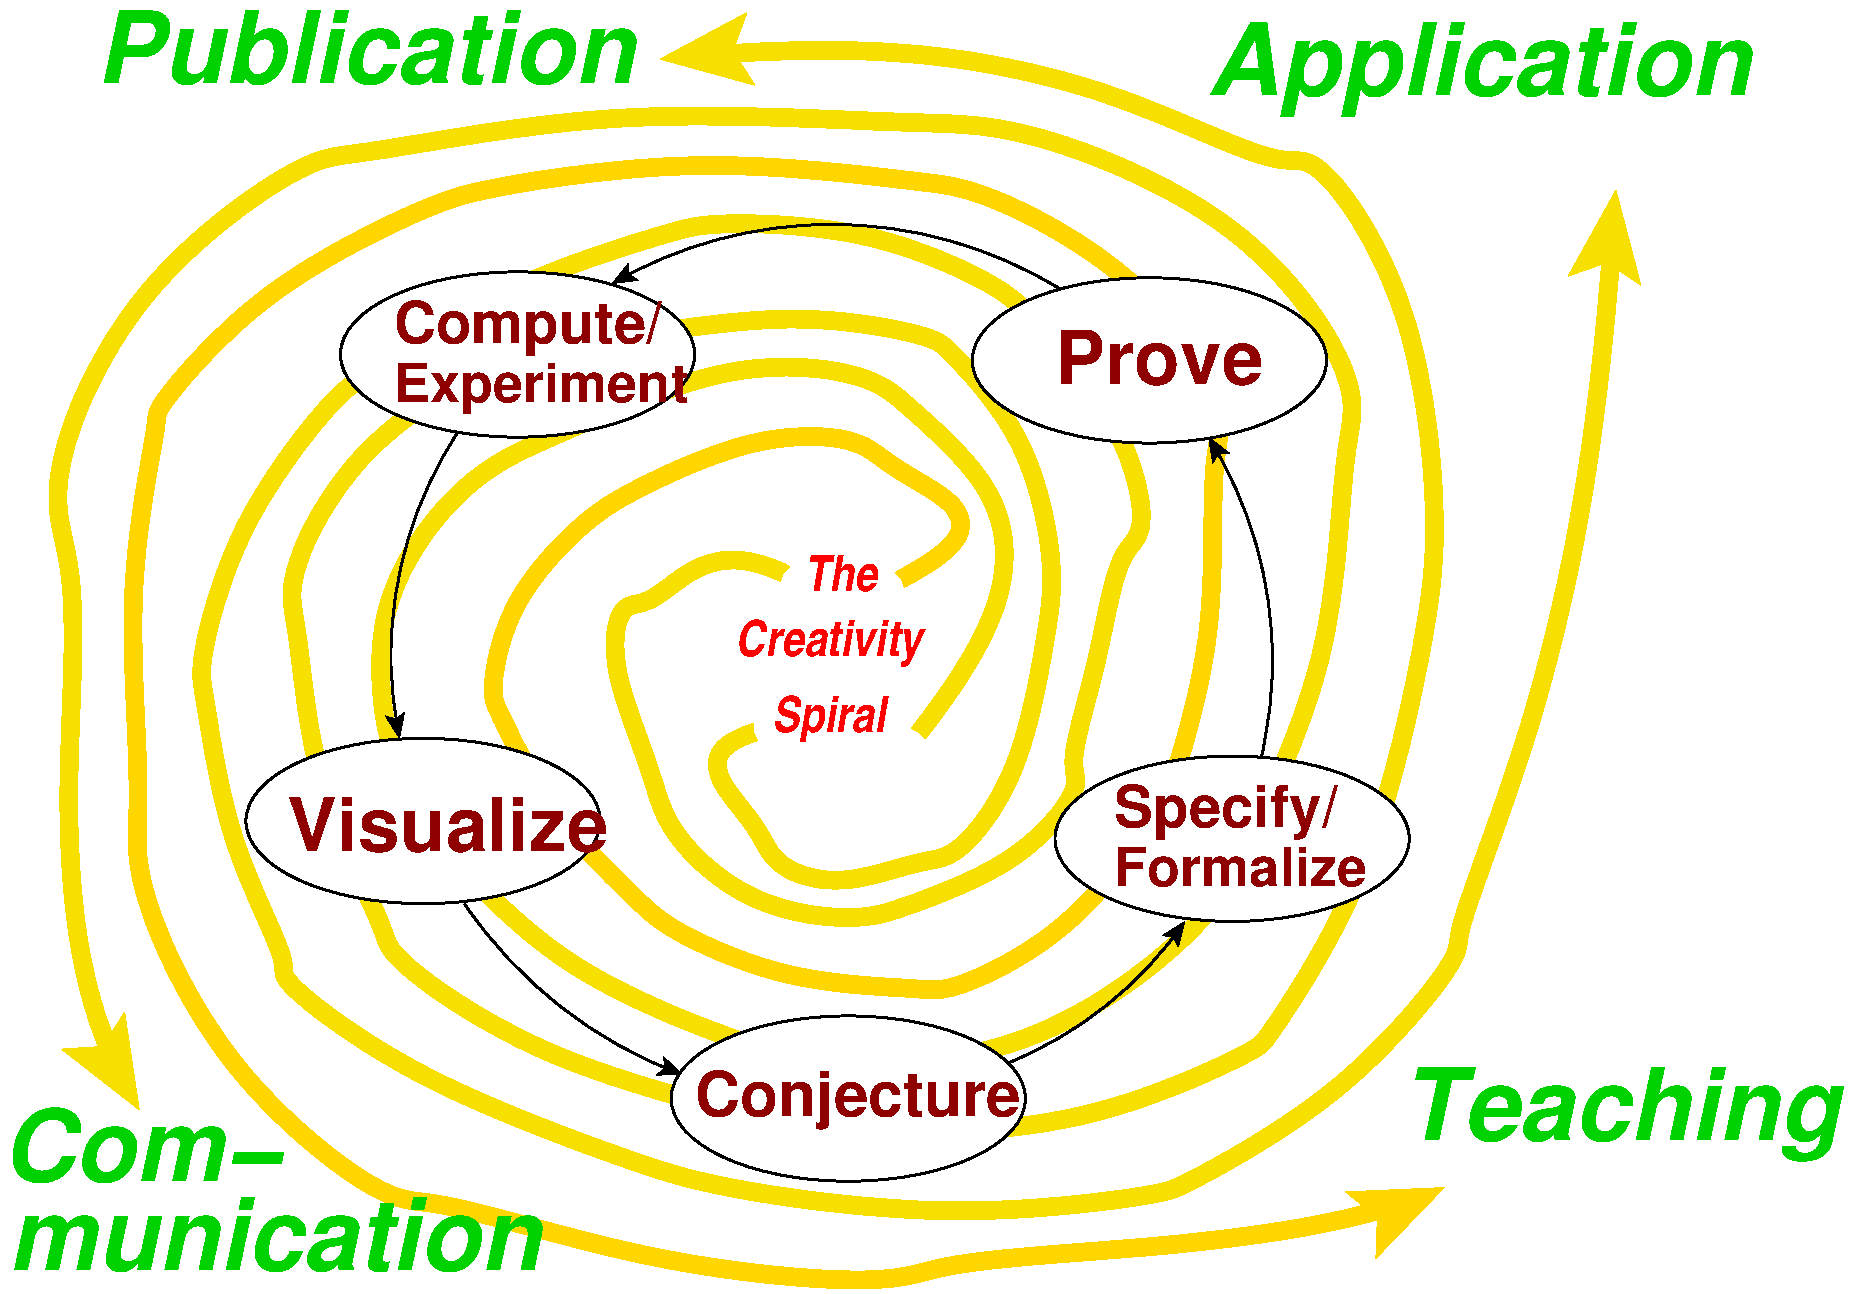
\includegraphics[width=\textwidth]{images/creativity-spiral}};
    \node at (s.south) {\scriptsize (B.\ Buchberger, 1995)};
  \end{tikzpicture}
      \end{column}
    \end{columns}
\end{frame}

\begin{frame}
  \frametitle{The Kepler Conjecture}
  \begin{center}
      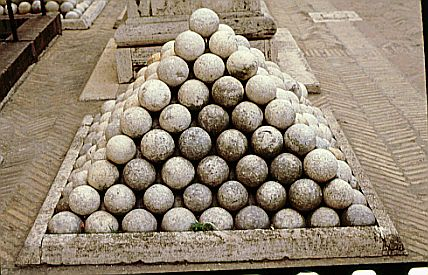
\includegraphics[width=.3\textwidth]{images/cannonballs.jpg}
  \end{center}
  \vspace{-1ex}
      \begin{itemize}
      \item 1611: Kepler conjectures that the max.\ density of packed unit
        spheres in 3D is $\pi/(3\sqrt{2})$
      \item 19??: Hilbert includes the conjecture in his 18\textsuperscript{th} problem
      \item 1995: Hales proves the conjecture with massive computer usage:
        \begin{itemize}
        \item 300 pages of human-readable text (theoretical foundations, proof outline)
        \item thousands of lines of computer code (non-standard, not formalized
          for a proof assistant)
        \item touches many areas of mathematics: plane, solid, spherical
          geometry, graph theory, hypermaps, single and multibariable calculus,
          plane and spherical trigonometry
        \end{itemize}
      \end{itemize}
\end{frame}

\begin{frame}
  \frametitle{Flyspeck}
  \begin{itemize}
  \item 1995: Hales proves the Kepler conjecture
  \item Reviewers are 99\% convinced but cannot verify the proof
  \item 2003: Hales initiates the \textbf{F}lys\textbf{p}ec\textbf{k} project to
    fully formalize (``computerize'') the proof to a proof assistant's level
  \item Expected duration: 20 man-years
  \end{itemize}
  Intermediate results of computerization:
  \begin{itemize}
  \item one fundamental algorithm in the computer code proven correct
  \item linear programming and global optimization code being investigated in
    two Ph.\,D.\ theses
  \end{itemize}
  Bulk of mathematical formalization remains to be done:
  \begin{itemize}
  \item elementary theories (e.\,g.\ spherical geometry) need to be defined\\
    (existing proof assistant libraries don't contain them!)
  \item then the specific aspects of Kepler
  \end{itemize}
\end{frame}

\begin{frame}
  \frametitle{Supporting Flyspeck in a Wiki}
  \begin{itemize}
  \item Flyspeck makes an excellent use case for a semantic wiki
  \item Not only the highly formal proof is the goal, but also
    human-comprehensible description
  \item Large number of loosely coupled lemmas $\Rightarrow$ many people can
    collaborate independently
  \end{itemize}
  Requirements for a wiki:
  \begin{itemize}
  \item human-readable presentation of descriptive text
  \item support for stepwisely computerizing human-readable informal text
  \item support for additional annotations, e.\,g.\ for discussing a formal
    definition, or for project management
  \item import/export interface to proof assistant(s), ultimately having the
    proof assistant integrated into the wiki (cf.\ MathWiki)
  \end{itemize}
\end{frame}

\newcommand{\wikipage}[6]{\node[draw,text width=4cm,font=\tiny\sffamily,#6] (#1) at #2 {
    {\scriptsize\bfseries #3}\\
    #4
    ~\\[.5em]
    [Download computerization]\\
    #5
  };}
\newcommand{\dummywikipage}[2]{\wikipage{#1}{#2}{\textcolor{red!20}{Cosine}}{\textcolor{red!20}{$\cos$}}{
      \textcolor{red!20}{Page type: Definition\\
      Topic: Trigonometry}
    }{fill=red!20}}

\begin{frame}
  \frametitle{Scenario}
  \begin{enumerate}
  \item Browse for to-dos
  \item Download (with dependencies) into local proof checker
  \item Browse wiki for help, discuss existing formalizations, refine informal
    annotations
  \item Upload computerized proof, wiki checks it
  \end{enumerate}
\vspace{-2ex}
  \begin{center}
      \begin{tikzpicture}[set style={{default}+=[xscale=1.5,yscale=1.2,font=\sffamily]},default,xscale=.8]
    \fill[red!20] (-2.0,-1.0) rectangle (8.1,1.0);
    \wikipage{lemma}{(0,0)}{Lemma 1.3}{The cosine is an even function.\\
      The sine is an odd function.\\
      ${\color{blue}\underline{\cos}}(-x)={\color{blue}\underline{\cos}}(x)$\\
      ${\color{blue}\underline{\sin}}(-x)=-{\color{blue}\underline{\sin}}(x)$}{Type:
      Lemma, Topic: Trigonometry\\
      Proven: no (3 attempts)}{fill=red!20}
    \dummywikipage{tan}{(6.2,-0.2)}
    \draw[black!75] (lemma) -- (tan);
    \dummywikipage{sin}{(6.1,-0.1)}
    \draw[black!75] (lemma) -- (sin);
    \wikipage{cos}{(6,0)}{Cosine}{$\cos\colon{\color{blue}\underline{\mathbb{R}}}\to{\color{blue}{\underline{\mathbb{R}}}},x\mapsto\ldots$}{
      Page type: Definition\\
      Topic: Trigonometry
    }{fill=red!20}
    \wikipage{todo}{(0,2.2)}{To do}{%
      \begin{tabular}{l|l|l}
        Topic & Lemma & Discussion \\
        \hline
        Trigonometry & \textcolor{blue}{\underline{1.3}} & 5 posts \\
        Hypermaps & 4.2 & \ldots 
      \end{tabular}
    }{
      Type: Overview
    }{}
    \node at (2.7,2.7) {\textcolor{blue}{\underline{1. Browse}}};
    \node[fill=red!20] (d) at (3.5,1.8) {2. Download};
    \draw[->,thick,red!50] (lemma.north east) -- (d);
    \draw[->] (lemma) -- node[above] {usesSymbol} (cos);
    \draw[->] (todo) -- node[left] {references} (lemma);
  \end{tikzpicture}
  \end{center}
\end{frame}

\begin{frame}
  \frametitle{Wiki Structure}
  \begin{itemize}
  \item Knowledge base: one page contains one theory, symbol definition,
    lemma, or proof
  \item One discussion page per knowledge item, discuss issues related to the
    knowledge item there
  \item Theory browser: browse e.\,g.\ by topic (``spherical geometry''), or by
    logical dependency
  \item Editor: annotate and structure semi-formal texts, refactor definitions
    and theories
  \item Download (with dependencies), Upload (with check)
  \item Query interface:
    \begin{itemize}
    \item ``Which lemmas about composite regions need to be proved?''
    \item ``What lemmas are difficult to prove?''
    \item ``What do I need to understand the Jordan Curve Theorem?''
    \item ``What other lemmas could help me to prove this one?''
    \end{itemize}
  \end{itemize}
\end{frame}
\begin{frame}
  \frametitle{Evaluation of two Wikis}
  What is the right wiki to support Flyspeck?
  \begin{itemize}
  \item Data at our disposal: 
    \begin{itemize}
    \item the \TeX\ sources of the Flyspeck outline
    \item a Twelf computerization of lemmas from trigonometry
    \end{itemize}
  \item Imported these into Semantic MediaWiki and SWiM
  \item Evaluated how much of the Flyspeck requirements these existing systems
    fulfilled
  \end{itemize}
\end{frame}

\begin{frame}
  \frametitle{Semantic MediaWiki}
  \begin{itemize}
  \item imported Twelf computerization via a custom upload page, enhanced it to
    improve navigation (symbols linked to their declaration, automatic
    categorization)
  \item one page for every computerized lemma, transcluded into one with
    additional comments and annotations
  \item Queries easy but not powerful enough (e.\,g.\ no negation):
    \texttt{[[Category:Unproven]] [[Category:Lemma]] [[Category:Trigonometry]]
      [[written in::Twelf]]}
  \item Ad hoc ontology development found useful for project management
  \item Importing existing OMDoc ontology for mathematical knowledge: could
    merely reuse vocabulary, no inference supported
  \item \LaTeX\ formulæ not semantically structured
  \end{itemize}
\end{frame}

\begin{frame}
  \frametitle{Semantic MediaWiki}
  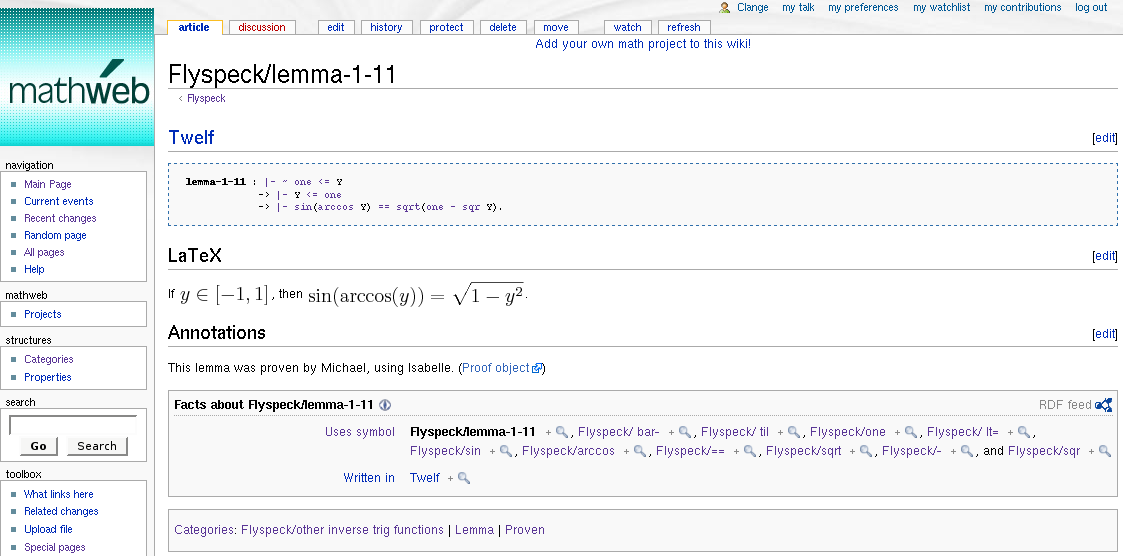
\includegraphics[width=\textwidth]{images/smw-lemma}
\end{frame}

\begin{frame}[fragile]
  \frametitle{SWiM}
  \begin{itemize}
  \item Manually converted some Twelf to OMDoc, SWiM's native math
    representation language (like OpenMath, but more expressive)\\
    (Automated conversion possible, too)
  \item SWiM supports OMDoc's ontology: types of mathematical knowledge items
    and their interrelations, e.\,g.\ ``Proof proves Assertion''
  \item Structured discussion pages: infrastructure for issue tracking and
    resolving (work in progress)
  \item SPARQL inline queries:
\begin{lstlisting}
SELECT ?l WHERE { ?l rdf:type odo:Lemma .
                  ?l swrc:isAbout <Composite_Regions> .
                  OPTIONAL { ?p rdf:type odo:Proof .
                             ?p odo:proves ?l . }
                  FILTER ( ! bound(?p) ) }
\end{lstlisting}
    \item Annotation not as straightforward as in Semantic MediaWiki
    \item Good RDF-based browsing, graph browser
    \item Reasoning powerful in principle (Pellet DL reasoner), but doesn't scale
    \item Semantically structured mathematical formulæ
  \end{itemize}
\end{frame}

\begin{frame}
  \frametitle{SWiM}
  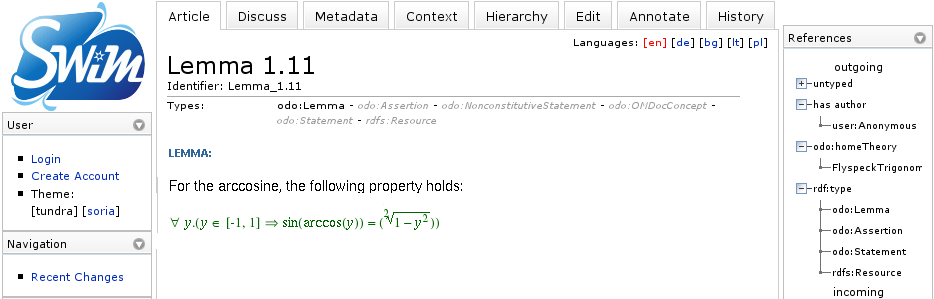
\includegraphics[width=\textwidth]{images/swim-lemma}

\end{frame}

\begin{frame}
  \frametitle{Related Work}
  \begin{itemize}
  \item Combining computerized proofs and human-readable text: Isar, Mizar (but
    no web collaboration)
  \item Informal mathematical knowledge collections: Wikipedia, PlanetMath (no
    semantics)
  \item Wikis integrating proof assistants:
    \begin{itemize}
    \item Logiweb: collaborative system, but hardly any browsing support.
      Interesting but idiosyncratic proof checker
    \item ProofWiki prototype: Coq proof assistant inside MediaWiki; so far no
      semantics except Coq's, content either computerized or human-readable
    \end{itemize}
  \end{itemize}
\end{frame}

\begin{frame}
  \frametitle{Conclusion and Further Work}
  Continue enabling SWiM for Flyspeck (but Semantic MediaWiki was great
    for rapid prototyping!)
  \begin{description}
  \item[Importing:] need to investigate existing \LaTeX $\to$ HTML+MathML path,
    extend towards OMDoc, use SWiM's split-on-import
  \item[Annotating:] need more flexibility; need refactoring assistance
  \item[Browsing:] narrative book structure would be important for humans.  Work
    aligning OMDoc and SALT ontologies in progress.
  \item[Discussing:] integrating DILIGENT argumentation ontology with
    domain-specific extensions into SWiM
  \item[Querying:] formula search not investigated, but solution exists.
    E.\,g.\ retrieve $\int_0^\infty f(y+z)dy$ by searching $\int_?^? f(x ? z)dz$
  \item[Different PAs:] For now focus on a single proof assistant (likely
    Isabelle), but logic translation would be nice
  \item[Download:] computing dependencies: rules could work, but probably need a
    more sophisticated calculus
  \item[Upload:] integrating theorem prover for checking uploaded data
  \end{description}
\end{frame}
\end{document}
